{\textbf{1. 二叉树的定义}}

{二叉树首先是一棵树。再附加两个限制条件:}

{{条件一:} 每个结点最多只有两个子树,即二叉树中结点的度只能为0、1、2。}

{{条件二:}子树有左右之分。}{}

{\textbf{2. 满二叉树}}

{在一棵二叉树中,{如果所有的分支结点都有左孩子和右孩子结点,并且叶子结点都集中在二叉树的最后一层},这样的二叉树称为满二叉树,见下图。}

{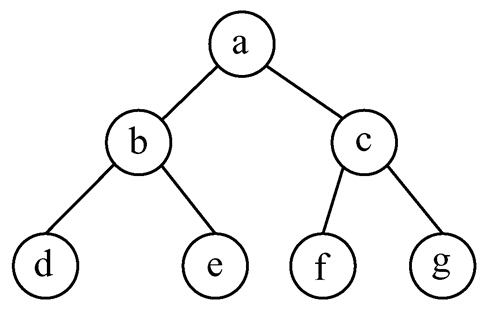
\includegraphics[width=2.08333in,height=2.08333in]{png-jpeg-pics/2168d1522cee5397fd408c62e74e19f7?}\\
\hspace*{0.333em}}

{\textbf{3. 完全二叉树}}

{若设二叉树的深度为h,除第h层外,其他各层(1~h-1)的结点数都达到最大个数,{第h层所有的结点都连续集中在最左边},这就是完全二叉树,见下图。}

{}

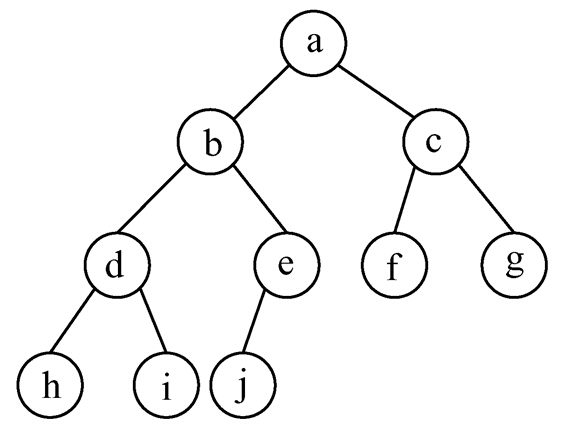
\includegraphics[width=2.08333in,height=2.08333in]{png-jpeg-pics/db52833b3034c215c5d5ec6e8ac982ed?}
